\begin{figure}[h]
\centering
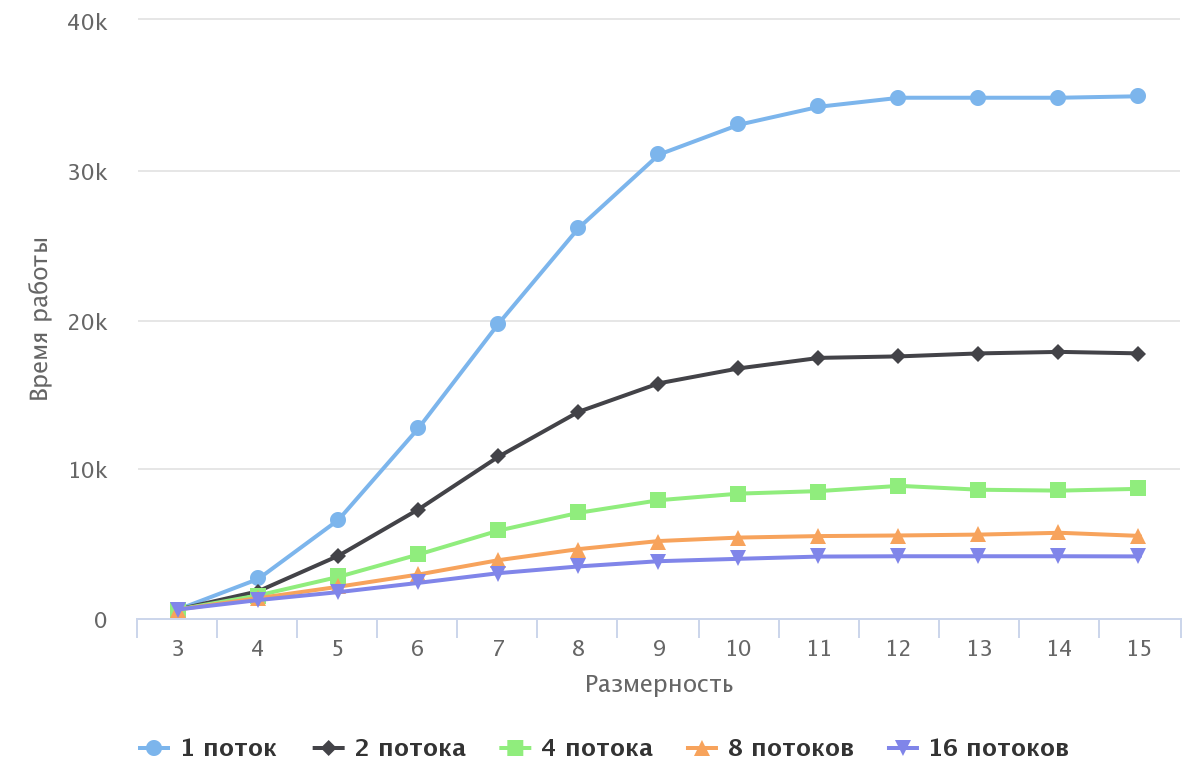
\includegraphics[width=\textwidth]{images/100k.png}
\caption{Медианное время работы при $N=10^5$}
\label{pic1}
\end{figure}

По полученным результатам видно, что при больших $N$ достигается неплохой уровень параллелизма.

\begin{table}[h]
\caption{Время работы алгоритма при $N=10^5$}\label{tab1}
\centering
\begin{tabu}{|*{8}{c|}}
\hline
 & \multicolumn{3}{c|}{Original} & \multicolumn{4}{c|}{Parallel 16 threads}\\
\cline{2-8}
    M & min & max & med & min & max & med & $t_1/t_2$ \\
\hline
    3 & 5.66e+02 & 5.70e+02 & 5.68e+02 & 5.67e+02 & 5.73e+02 & 5.70e+02 & \textbf{1.00}\\ 
    4 & 2.50e+03 & 2.82e+03 & 2.61e+03 & 1.13e+03 & 1.27e+03 & 1.20e+03 & \textbf{2.16}\\
    5 & 6.46e+03 & 6.80e+03 & 6.56e+03 & 1.67e+03 & 1.89e+03 & 1.73e+03 & \textbf{3.79}\\
    6 & 1.26e+04 & 1.28e+04 & 1.27e+04 & 2.28e+03 & 2.45e+03 & 2.35e+03 & \textbf{5.40}\\
    7 & 1.96e+04 & 1.99e+04 & 1.97e+04 & 2.93e+03 & 3.06e+03 & 3.00e+03 & \textbf{6.57}\\
    8 & 2.59e+04 & 2.62e+04 & 2.61e+04 & 3.30e+03 & 3.57e+03 & 3.45e+03 & \textbf{7.57}\\
    9 & 3.08e+04 & 3.12e+04 & 3.10e+04 & 3.69e+03 & 3.91e+03 & 3.80e+03 & \textbf{8.16}\\
    10& 3.28e+04 & 3.32e+04 & 3.30e+04 & 3.85e+03 & 4.03e+03 & 3.96e+03 & \textbf{8.33}\\
    11& 3.41e+04 & 3.45e+04 & 3.42e+04 & 3.99e+03 & 4.24e+03 & 4.11e+03 & \textbf{8.32}\\
    12& 3.46e+04 & 3.51e+04 & 3.48e+04 & 3.98e+03 & 4.25e+03 & 4.13e+03 & \textbf{8.43}\\
    13& 3.46e+04 & 3.51e+04 & 3.48e+04 & 4.00e+03 & 4.36e+03 & 4.13e+03 & \textbf{8.43}\\
    14& 3.46e+04 & 3.50e+04 & 3.48e+04 & 4.01e+03 & 4.43e+03 & 4.13e+03 & \textbf{8.43}\\
    15& 3.47e+04 & 3.52e+04 & 3.49e+04 & 3.95e+03 & 4.25e+03 & 4.12e+03 & \textbf{8.47}\\
\hline
\end{tabu}
\end{table}
